%%%%%%%%%%%%%%%%%%%%%%%%%%
% USFD Academic Report Template
% Prof. Roger K. Moore
% University of Sheffield
% 30 July 2018
% Adapted by Loïc Barrault
% 16 September 2021
% Adapted by Yu Chen
% 10/05/2024
%%%%%%%%%%%%%%%%%%%%%%%%%%
%%%%%ATTETION%%%%%%%%%%%%%%%%%%%%%%%%%%
%%use XeLatex as complile engine
%%use BibTeX as the bibliography engine
%%%%%%%%%%%%%%%%%%%%%%%%%%%%%%%%%%%%%%%

\documentclass[12pt,oneside,french]{book}
\usepackage[utf8]{inputenc}
\usepackage{lmodern}
\usepackage{xeCJK}
%Windows系统用这个
\setCJKmainfont{SimSun}
%苹果系统用这个
%\setCJKmainfont{Songti TC}
\usepackage{tikz}
\usepackage{url}  % 让 URL 或 DOI 自动换行
\usepackage{tipa}
\usepackage{alltt}
\usepackage[margin=1.2in]{geometry}
\usepackage[toc,page]{appendix}
\usepackage{graphicx}
\usepackage[style=apa]{biblatex}
\usepackage{lipsum}
\usepackage{tabularx}  
\usepackage{svg}
\usepackage{hyperref}
\usepackage[T1]{fontenc}
\usepackage[french]{babel}
\usepackage{float}
\usepackage{caption}
\usepackage[toc,xindy]{glossaries}
\usepackage[automake]{glossaries-extra}
\usepackage{listings}

\usepackage{fontspec}
\setmainfont{Times New Roman}
\usepackage{setspace}
\onehalfspacing
% glossary.tex
\newglossaryentry{latex}
{
	name=LaTeX,
	description={A document preparation system}
}

\newglossaryentry{glossaries}
{
	name=Glossaries,
	description={A LaTeX package for creating glossaries}
}

% 定义更多的词汇条目
\makeglossaries
\addbibresource{main.bib}


\begin{document}
	\pagestyle{plain}

	\captionsetup[figure]{margin=1.5cm,font=small,labelfont={bf},name={Figure},labelsep=colon,textfont={it}}
	\captionsetup[table]{margin=1.5cm,font=small,labelfont={bf},name={Tableau},labelsep=colon,textfont={it}}
	\SetLipsumDefault{1}

\frontmatter

\begin{titlepage}
	
	
% -------------------------------------------------------------------
% You need to edit the details here
% -------------------------------------------------------------------

\begin{center}

\includegraphics[width=9cm]{images/logo.png}\\[1cm]
\linespread{1.2}\huge {\bfseries Titre}\\[1.5cm]
\linespread{1}
{\Large HERE IS YOUR NAME}\\[1cm]
{\large \emph{Sous la direction de :} Nom de l'encadrant}\\[1cm] % if applicable
{\large  \emph{Laboratoire :} YOUR LABORATOIRE}\\[1cm]  
{\large
UFR SHS\\
Départment Mathématiques et informatique appliquées aux sciences humaines et sociales\\% change as necessary
\today}
\end{center}
\end{titlepage}


% -------------------------------------------------------------------
% Declaration
% -------------------------------------------------------------------

\newpage
%! Author = Yu
%! Date = 2024/6/13


\section*{\Large Déclaration}

Toutes les phrases et passages cités dans ce document provenant de travaux d'autres personnes ont été spécifiquement identifiés par une citation claire à l'auteur, le travail et la ou les pages correspondantes.
Toutes les illustrations qui ne sont pas le travail de l'auteur de ce rapport sont utilisées avec l'accord de leur auteur et sont également clairement référencées. Je comprends que faillir à cela équivaut à du plagiat et sera considéré en tant que tel lors de l'évaluation.\\[1cm]

\noindent Prénom NOM: \\[1mm]
\rule[1em]{25em}{0.5pt}

\noindent Date: \today \\[1mm]
\rule[1em]{25em}{0.5pt}

\noindent Signature:\\[1mm]
% \includegraphics[width=4.5cm]{images/electronic_name.png}
\\
\rule[1em]{25em}{0.5pt}
% -------------------------------------------------------------------
	% Abstract
	% -------------------------------------------------------------------


% -------------------------------------------------------------------
% Abstract
% -------------------------------------------------------------------

\newpage
\section*{\Large \center Résumé}
% Guidance of how to write an abstract/summary provided by Nature: https://cbs.umn.edu/sites/cbs.umn.edu/files/public/downloads/Annotated_Nature_abstract.pdf

Une ou deux phrases présentant une introduction générale du domaine, compréhensible par des scientifiques non spécialistes du domaine.
Deux à trois phrase sur le contexte plus spécifique du projet, compréhensible par des scientifiques spécialisés dans des disciplines liées.
Une phrase présentant clairement le problème adressé par ce travail.
Une phrase résumant le résultat principal de travail effectué.
Deux ou trois phrases expliquant ce que révèle ce résultat sur l'état de l'art actuel ou ce qu'il ajoute aux connaissances antérieures.
Une ou deux phrases pour mettre les résultats dans un contexte plus global.
Deux ou trois phrases d'ouverture vers des travaux futurs, compréhensibles par des scientifique de toute discipline.


\section*{\Large \center Abstract}
\lipsum

\newpage


% -------------------------------------------------------------------
% Contents, list of figures, list of tables
% -------------------------------------------------------------------

\tableofcontents
\listoffigures
\listoftables


% -------------------------------------------------------------------
% Main sections (as required)
% -------------------------------------------------------------------

\mainmatter

%! Author = Yu
%! Date = 2024/5/30

\chapter*{Introduction}
\addcontentsline{toc}{chapter}{Introduction}
\lipsum
\chapter{État de l'art}

\section{Une section contenant des référence}

Selon le travail fondateur de \cite{Reference1}, lorem ipsum dolor sit amet.  
Cependant, ce résultat était déjà connu depuis les années 1990 \cite{Reference2,Reference3}.  
% Note the use of \cite{} and \citep{}


\section{Une section contenant des mathématiques}

\lipsum  % Remplacer avec votre texte
 
\begin{equation}
M = \frac{1}{T}\sum_{t=1}^{T} e(t) / \max_{t}[e(t)]
\label{eq:equation}
\end{equation}

\lipsum  % Remplacer avec votre texte

Cela est montré dans l'\autoref{eq:equation} et est répété ici en ligne $M = \frac{1}{T}\sum_{t=1}^{T} e(t) / \max_{t}[e(t)]$.


\section{Une section contenant une figure}

\lipsum  % Remplacer avec votre texte

\begin{figure}[ht]
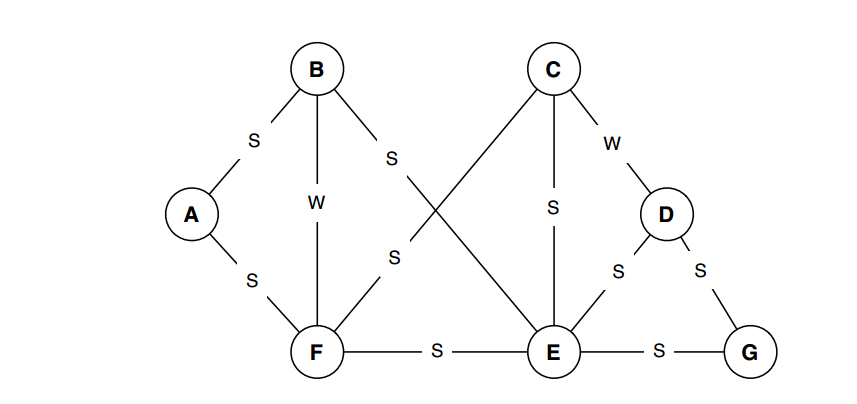
\includegraphics[width=15cm]{figures/figure1.png}
\caption{Une figure simple en \LaTeX. Issue de http://tinyurl.com/nqtrlj5.}
\label{fig:graph}
\end{figure}

\lipsum  % Remplacer avec votre texte

Voir \autoref{fig:graph}.


\section{Une section contenant un tableau}

\lipsum  % Remplacer avec votre texte

\begin{table}[ht]
\center
\begin{tabular}{cc|c}
A & B & A XOR B\\
\hline
0 & 0 & 0\\
0 & 1 & 1\\
1 & 0 & 1\\
1 & 1 & 0\\
\end{tabular}
\caption{Un tableau très simple en \LaTeX.}
\label{tab:xor}
\end{table}

\lipsum  % Remplacer avec votre texte

Cela est montré dans le \autoref{tab:xor}.


\section{Résumé}

\lipsum  % Remplacer avec votre texte

\chapter{Méthodologie}
\lipsum  % Remplacer avec votre texte


\section{section 1}

\lipsum  % Remplacer avec votre texte


\section{section 2}

\lipsum  % Remplacer avec votre texte


\chapter{Résultats}

\section{Résultats 1}

\lipsum  % Remplacer avec votre texte


\section{Résultats 2}

\lipsum  % Remplacer avec votre texte

\chapter{Discussion}

\lipsum  % Remplacer avec votre texte

\chapter*{Conclusion}
\addcontentsline{toc}{chapter}{Conclusion}
\lipsum
\lipsum  % Remplacer avec votre texte


% -------------------------------------------------------------------
% Bibliography
% -------------------------------------------------------------------

\sloppy
\printbibliography
\addcontentsline{toc}{chapter}{Bibliographie}
\printglossary[title={Glossaire},toctitle={Glossaire}]
% -------------------------------------------------------------------
% Appendices
% -------------------------------------------------------------------

\begin{appendices}
\chapter{Un premier appendice}

\lipsum[1-3]  % Remplacer avec votre texte

\chapter{Un second appendice}

\lipsum[1-3]  % Remplacer avec votre texte

\end{appendices}
\end{document}